\section{Expressões regulares}

\begin{frame}[allowframebreaks,fragile]
\frametitle{Expressões regulares}

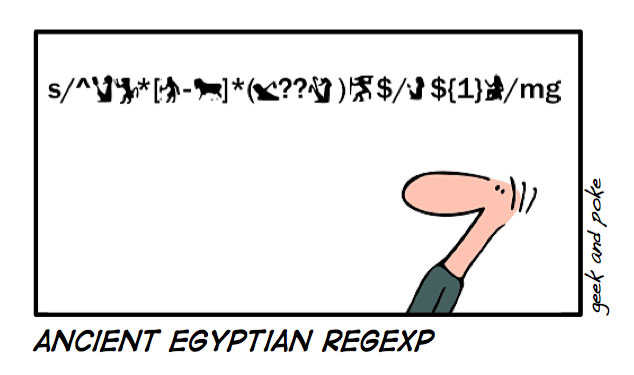
\includegraphics[width=0.6\textwidth,height=0.5\textheight,keepaspectratio]{figures/regexp01.jpg}

\framebreak

Expressão regular (regex ou regexp) provê uma forma concisa e flexível de identificar
padrões de interesse, como caracteres particulares, palavras ou sequências de
caracteres. Expressões regulares são escritas numa linguagem formal que será
interpretada por um processador de expressão regular.

Expressão regular deriva do trabalho do matemático norte-americano Stephen Cole Kleene,
que desenvolveu as expressões regulares como uma notação ao que ele chamava de álgebra
de conjuntos regulares. Seu trabalho serviu de base para os primeiros algoritmos
computacionais de busca, e depois para algumas das mais antigas ferramentas de tratamento
de texto da plataforma Unix.

\framebreak

Uma expressão regular (ou, um padrão) descreve um conjunto de cadeias de caracteres,
de forma concisa, sem precisar listar todos os elementos do conjunto.
Para realizar esta tarefa, as expressões regulares são descritas utilizando uma
determinada sintaxe e um determinado alfabeto de símbolos, cada qual com o seu significado
específico.

\framebreak

Veremos exemplos de expressões regulares utilizando o \texttt{grep}.

Para os exemplos a seguir, utilizaremos o texto \emph{Alice no País das Maravilhas} de Lewis Carroll.

\begin{lstlisting}[language=bash, label=lst-grep-prep, caption={Download do texto no Projeto Gutenberg.}, postbreak=\mbox{$\hookrightarrow$\space}, basicstyle=\fontsize{8}{10}\selectfont\ttfamily]
wget https://www.gutenberg.org/files/11/11-0.txt -O alice.txt
\end{lstlisting}

\framebreak

\begin{lstlisting}[language=bash, label=lst-grep-01, caption={Busca por um caractere ou uma sequência.}, postbreak=\mbox{$\hookrightarrow$\space}, basicstyle=\fontsize{8}{10}\selectfont\ttfamily]
# encontrar o caractere ? no texto
$ grep ? alice.txt

# encontrar a palavra King no texto
$ grep King alice.txt

# encontrar a palavra king no texto (sensível a diferença entre maiúsculas e minúsculas)
$ grep king alice.txt

# encontrar a palavra King ou king no texto
$ grep [Kk]ing alice.txt

# encontrar a palavra While ou while no texto
$ grep [Ww]hile alice.txt

# para que a busca seja insensível a maiúscuas ou minúsculas
$ grep -i king alice.txt
\end{lstlisting}

\framebreak

\begin{lstlisting}[language=bash, label=lst-grep-02, caption={O uso de colchetes representa uma disjunção de caracteres.}, postbreak=\mbox{$\hookrightarrow$\space}, basicstyle=\fontsize{8}{10}\selectfont\ttfamily]
# usando os colchetes para designar um dos caracteres w ou o
$ grep t[wo]o alice.txt

# encontrar qualquer sequência de 3 letras em que a primeira seja t e a última o
$ grep t[a-z]o alice.txt

# o mesmo, porém mostrar apenas os matches
$ grep -o t[a-z]o alice.txt

# contabilizar os padrões observados
$ grep -o t[a-z]o alice.txt | sort | uniq -c

# encontrar dígitos
$ grep [0-9] alice.txt
\end{lstlisting}

\framebreak

\begin{table}
\caption{meta caracteres - caracteres com significado especial}\label{tab-regex-metachar}
\begin{tabular}{ll}
caractere & significado \\
\midrule
$[$ $]$ &  classse de caracteres        \\ 
\textbackslash     &  caracteres especiais       \\ 
\^{}   &  negação                    \\ 
\$     &  fim da cadeia de caracteres\\ 
.      &  qualquer caractere         \\ 
|      &  uma expressão ou outra     \\ 
?      &  zero ou uma vez            \\ 
$\ast$ &  zero ou mais vezes         \\ 
+      &  uma ou mais vezes          \\ 
( )    &  captura de dados           \\ 
\end{tabular}
\end{table}

\begin{lstlisting}[language=bash, label=lst-grep-03, caption={}, postbreak=\mbox{$\hookrightarrow$\space}, basicstyle=\fontsize{8}{10}\selectfont\ttfamily]
# encontrar Alice no início de uma linha                                             
$ grep ^Alice alice.txt

# encontrar duas ocorrências de Alice em uma linha
$ grep -n Alice.*Alice alice.txt       

# encontrar Alice no final de uma linha
# (vamos remover os 'carriage returns' presentes no texto)
$ cat alice.txt | tr -d '\r' | grep Alice$
\end{lstlisting}

\framebreak

\begin{table}
\caption{Abreviações para classes de caracteres.}\label{tab-regex-charpat}
\begin{tabular}{ll}
padrão & significado \\
\midrule
\textbackslash s  &    espaços em branco, \textbackslash n \textbackslash r ou \textbackslash t \\                   
\textbackslash S  &    negação de \textbackslash s, tudo o que não for espaço em branco \\
\textbackslash w  &    letras, dígitos, ou '\textbackslash\_'         \\
\textbackslash W  &    negação de \textbackslash w                    \\
\textbackslash d  &    dígitos, de 0 a 9                 \\
\textbackslash D  &    negação de \textbackslash d                    \\
\end{tabular}
\end{table}

\framebreak

\begin{lstlisting}[language=bash, label=lst-grep-04, caption={Abreviações para classes de caracteres.}, postbreak=\mbox{$\hookrightarrow$\space}, basicstyle=\fontsize{8}{10}\selectfont\ttfamily]
# encontrar Alice seguida de um símbolo que não seja \s (espaço, quebra de linha ou tabulação), ao final contabilizar os padrões presentes
$ grep Alice\\S -o alice.txt | sort | uniq -c | sort -rn

# encontrar números
$ grep '[0-9]\+' alice.txt
$ grep '[[:digit:]]' alice.txt
$ grep -P '\d+' alice.txt
$ grep -P '\D\d{4}\D' alice.txt

# encontrar números de telefone
$ grep -P '\(?\+?\d{1,3}\)?[\s\-]\d{3,4}[\s\-]\d{3,4}' alice.txt
\end{lstlisting}

\framebreak


\begin{table}
\caption{Marcadores para indicar repetições.}\label{tab-regex-rep}
\begin{tabular}{ll}
símbolo & significado \\
\midrule
$\ast$      &   nenhum ou qualquer número de repetições       \\ 
$+$         &   uma ou mais repetições                        \\
\{min,max\} &   indica o número mínimo e máximo de repetições \\
\{2,4\}     &   de 2 a 4 repetições                           \\
\{0,\}      &   equivalente ao *                              \\
\{1,\}      &   equivalente ao +                              \\
\end{tabular}
\end{table}


\framebreak

\begin{lstlisting}[language=bash, label=lst-grep-05, caption={Outros exemplos com repetições.}, postbreak=\mbox{$\hookrightarrow$\space}, basicstyle=\fontsize{8}{10}\selectfont\ttfamily]
# encontrar sequências de 3 dígitos
$ grep -P '\d{3}' alice.txt

# encontrar sequências com 2 ou mais dígitos
$ grep -P '\d{2,}' alice.txt

# encontrar uma sequência composta de dois caracteres seguidos por 'cept'
$ grep '..cept' alice.txt  

# encontrar qualquer sequência terminada em 'ime' que não seja 'time' ou 'Time'
$ grep "[^t^T]ime" alice.txt

# encontrar um trecho entre parênteses
$ grep '([A-Za-z ]*)' alice.txt

# encontrar uma sequência de letras ou espaço seguida de uma sequência de dígitos
# (-P, --perl-regexp, Perl-compatible regular expression)
$ grep -P '[\w\s]+\d+' alice.txt 

# procura pela palavra heart ou hearts usando s opcional e \b limitador de palavras
$ grep -i '\bhearts\?\b' alice.txt

# encontrar três vogais quaisquer em sequência
$ grep -i '[aeiou]\{3\}' alice.txt
\end{lstlisting}


\framebreak

\begin{lstlisting}[language=bash, label=lst-grep-06, caption={Contexto.}, postbreak=\mbox{$\hookrightarrow$\space}, basicstyle=\fontsize{8}{10}\selectfont\ttfamily]
# mostra o contexto onde está a palavra clock (3 linhas antes e 2 após)
$ grep -B3 -A2 clock alice.txt

# procura pelas strings clock e watch (note que achará watch em watching e watched)
# -E, --extended-regexp
$ grep -E 'clock|watch' alice.txt

# procura pelas palavras clock e watch (usando o delimitador de palavras \b)
$ grep -E '\bclock\b|\bwatch\b' alice.txt

# outra opção é utilizar \< e \> para delimitar palavras
$ grep '\<cat\>' alice.txt 

# encontra uma palavra qualquer que aparece duas vezes na mesma linha
$ grep '\b\(\w\+\)\b.*\b\1\b' alice.txt 

# encontrar palavras que começam e terminam com vogais
$ grep -i '\b[aeiou]\w\+[aeiou]\b' alice.txt
$ grep -iE '\b[aeiou]\w+[aeiou]\b' alice.txt 
$ egrep -i '\b[aeiou]\w+[aeiou]\b' alice.txt

# ideem
# (-o or --only-matching)
$ grep -io '\b[aeiou]\w\+[aeiou]\b' alice.txt

# mostra lista (sem repetições) e insensível a maiúsculas
$ grep -io '\b[aeiou]\w\+[aeiou]\b' alice.txt | tr 'A-Z' 'a-z' | sort | uniq

# encontrar palavras compostas
# (note que não faz match com palavras compostas com mais de 2 palavras)
$ grep -i '[a-z]\+\-[a-z]\+' alice.txt

# mostrar as palavras compostas encontradas
# agora consideranto palavra composta com 2 ou mais palavras
$ grep -io '[a-z]\+\(\-[a-z]\+\)\+' alice.txt | tr 'A-Z' 'a-z' | sort | uniq

# listar as palavras que possuem três vogais em sequência
$ grep -io '\b\w\+[aeiou]\{3\}\w\+\b' alice.txt  | tr 'A-Z' 'a-z' | sort | uniq

# listar palavras em que um caractere qualquer repete pelo menos 3 vezes
$ grep -io '\b\w*\(\w\)\1\{2,\}\w*\b' alice.txt

# outro exemplo da mesma funcionalidade
$ echo "lalala laaa la laa la laaaa laaam lam aaass" | grep -io '\b\w*\(\w\)\1\{2,\}\w*\b'

# listar palavras repetidas em sequência
$ grep -Ei '\<([A-Za-z]+) +\1\>' alice.txt 

# encontrar sequência entre aspas duplas
$ grep '"[^"]*"' alice.txt 
\end{lstlisting}

\framebreak
É possível  ainda colocar caracteres não imprimíveis em expressões regulares.

\begin{table}
\caption{Marcadores para caracteres não imprimíveis.}\label{tab-regex-npc}
\begin{tabular}{ll}
símbolo & significado \\
\midrule
\textbackslash r  &    carriage return (0x0D)          \\ 
\textbackslash n  &    line feed (0x0A)                \\
\textbackslash t  &    tab character (ASCII 0x09)      \\
\textbackslash a  &    (bell, 0x07)                    \\
\textbackslash e  &    (escape, 0x1B)                  \\
\textbackslash f  &    (form feed, 0x0C)               \\
\textbackslash v  &    (vertical tab, 0x0B)            \\
\end{tabular}
\end{table}


\begin{lstlisting}[language=bash, label=lst-grep-06, caption={Contexto.}, postbreak=\mbox{$\hookrightarrow$\space}, basicstyle=\fontsize{8}{10}\selectfont\ttfamily]
# verificar quantas linhas são terminadas com \r
$ grep -P '\r$' alice.txt | wc -l
\end{lstlisting}

\framebreak

Podemos ainda especificar um caractere pelo seu código hexadecimal ASCII ou ANSI.
Utilizamos para tanto \textbackslash x seguindo do código. 

\begin{table}
\caption{Alguns exemplos de uso do código hexadecimal para especificar caracteres.}\label{tab-regex-hex}
\begin{tabular}{ll}
símbolo & significado \\
\midrule
\textbackslash xA9 & copyright symbol    \\
\textbackslash x80 & Euro Sign           \\
\textbackslash xA3 & Pound Sign          \\
\textbackslash xB0 & Degree Sign         \\
...   &  ...                \\
\textbackslash x92 & non-ascii single quote \\
\textbackslash x93 & non-ascii open double quote \\
\textbackslash x94 & non-ascii close double quote\\
\end{tabular}
\end{table}

\framebreak

\begin{lstlisting}[language=bash, label=lst-grep-07, caption={Bucando aspas fora do padrão ASCII.}, postbreak=\mbox{$\hookrightarrow$\space}, basicstyle=\fontsize{8}{10}\selectfont\ttfamily]
# buscar pelas aspas fora do padrão ASCII
$ grep -P "\x22" alice.txt 
$ grep -P "\x27" alice.txt 

# utilizando o sed para substituir as aspas fora do padrão ASCII
$ sed -i "s/\x22/'/g" alice.txt 
$ sed -i 's/\x27/"/g' alice.txt 
\end{lstlisting}

\framebreak

\begin{quote}
Unfortunately, the regular expression language is no differ ent fr om any other in
that it has various dialects and accents. \cite{friedl_mastering_2006}
\end{quote}
\vspace{3ex}

\begin{quote}
When crafting a regular expression, you must consider the ongoing tug-of-war between having your expression
match the lines you want, yet still not matching lines you don’t want. \cite{friedl_mastering_2006}
\end{quote}


\end{frame}

\begin{frame}
\frametitle{Sugestão de leitura}

\fullcite{regular-expressions}
\vspace{2ex}

\fullcite{friedl_mastering_2006}
\vspace{2ex}

\fullcite{goyvaerts_regular_2012}

\end{frame}
